\documentclass{article}
\usepackage{nirav-ds203}
\usepackage{hyperref}  % Make sure this is loaded

\newcommand{\myname}{Nirav Bhattad}
\newcommand{\topicname}{DS203: Exercise 9}

\lstset{
    backgroundcolor=\color{gray!10}, % Set the background color
    numbers=left, % Display line numbers
    numberstyle=\ttfamily\tiny\color{gray}, % Set the style for line numbers
    breaklines=true, % Enable line breaking
    keepspaces=true, % Keep spaces in text
    keywordstyle=\color{blue}\bfseries, % Style for SQL keywords
    commentstyle=\color{green!50!black}, % Style for comments
    stringstyle=\color{red}, % Style for strings
    basicstyle=\ttfamily\footnotesize, % Set the font and size
    stepnumber=1, % Numbering every line
    tabsize=2, % Set tab size
    showspaces=false, % Do not display spaces
    showstringspaces=false, % Do not display string spaces
    showtabs=false, % Do not display tabs
    captionpos=b, % Position the caption at the bottom
    morekeywords={SELECT, FROM, WHERE, JOIN, INNER, LEFT, RIGHT, ON, GROUP, BY, ORDER, HAVING, UNION, INSERT, INTO, VALUES, UPDATE, SET, DELETE, CREATE, DROP, ALTER, DATABASE, TABLE, INDEX, UNIQUE, PRIMARY, FOREIGN, KEY, CONSTRAINT, AND, OR, NOT, BETWEEN, LIKE, IN, EXISTS, IS, NULL, DISTINCT, AS, LIMIT, OFFSET, OFFSET, CASE, WHEN, THEN, END, CAST, AS, COUNT, AVG, SUM, MIN, MAX, GROUP_CONCAT, COALESCE, NULLIF, SUBSTRING, LEFT, RIGHT, TRIM, LTRIM, RTRIM, CONCAT, IFNULL, CHAR_LENGTH, LENGTH, REPLACE, TRANSLATE, ROUND, CEIL, FLOOR, RAND, NOW, CURDATE, DATE, TIMESTAMP, CURRENT_DATE, CURRENT_TIME, CURRENT_TIMESTAMP, DATE_ADD, DATE_SUB, YEAR, MONTH, DAY, HOUR, MINUTE, SECOND, EXTRACT, YEAR, MONTH, DAY, WEEK, QUARTER, TO_DATE, TO_CHAR, USE},
    emph={SELECT, FROM, WHERE, JOIN, INNER, LEFT, RIGHT, ON, GROUP, BY, ORDER, HAVING, UNION, INSERT, INTO, VALUES, UPDATE, SET, DELETE, CREATE, DROP, ALTER, DATABASE, TABLE, INDEX, UNIQUE, PRIMARY, FOREIGN, KEY, CONSTRAINT, AND, OR, NOT, BETWEEN, LIKE, IN, EXISTS, IS, NULL, DISTINCT, AS, LIMIT, OFFSET, CASE, WHEN, THEN, END, CAST, COUNT, AVG, SUM, MIN, MAX, GROUP_CONCAT, COALESCE, NULLIF, SUBSTRING, LEFT, RIGHT, TRIM, LTRIM, RTRIM, CONCAT, IFNULL, CHAR_LENGTH, LENGTH, REPLACE, TRANSLATE, ROUND, CEIL, FLOOR, RAND, NOW, CURDATE, DATE, TIMESTAMP, CURRENT_DATE, CURRENT_TIME, CURRENT_TIMESTAMP, DATE_ADD, DATE_SUB, YEAR, MONTH, DAY, HOUR, MINUTE, SECOND, EXTRACT, YEAR, MONTH, DAY, WEEK, QUARTER, TO_DATE, TO_CHAR, USE, SHOW},
    emphstyle=\color{green!50!black}, % Make keywords green
    gobble=0, % No gobbling of characters
}

\begin{document}

\thispagestyle{empty}

\titleBC

\section*{Task 1}

\begin{task*}[1]
Do a manual review of the table \textbf{nsedata} and describe its contents
\end{task*}


The table \texttt{nsedata} contains daily stock market data for various companies. Each row in the table represents a stock identified by its symbol, detailing the performance during a specific trading session. The columns in the table are as follows:

\begin{longtable}{|l|l|l|}
\hline
\textbf{Column Name} & \textbf{Data Type} & \textbf{Description} \\
\hline
\endfirsthead
\hline
\textbf{Column Name} & \textbf{Data Type} & \textbf{Description} \\
\hline
\endhead
symbol & varchar(50) & Unique identifier for the stock/company (e.g., AAPL). \\
series & varchar(50) & Indicates the type of equity, all entries marked as EQ (common equity). \\
open & decimal(20,6) & The price at the start of the trading session. \\
high & decimal(20,6) & The highest price the stock reached during the day. \\
low & decimal(20,6) & The lowest price recorded during the day. \\
close & decimal(20,6) & The price at the end of the trading session. \\
last & decimal(20,6) & The last traded price, which may differ from the closing price. \\
prevclose & decimal(20,6) & The closing price from the previous trading session. \\
tottrdqty & int & The total traded quantity of the stock. \\
tottrdval & decimal(20,6) & The total traded value of the stock. \\
timestamp & varchar(50) & The timestamp of when the data was recorded. \\
anum & mediumint & An additional numeric field that may be used for internal purposes (nullable). \\
isin & varchar(50) & The International Securities Identification Number (nullable). \\
extra & varchar(50) & Any extra information related to the stock (nullable). \\
\hline
\end{longtable}

\textbf{Constraints:}
\begin{itemize}
    \item All columns, except \texttt{anum}, \texttt{isin}, and \texttt{extra}, are required to have non-null values.
    \item None of the columns are marked as keys.
    \item No default values have been set for any column.
\end{itemize}

\clearpage

\section*{Task 2}

\begin{task*}[2]
Select the database \textbf{stockdata} using SQL
\end{task*}

\begin{lstlisting}[language=SQL, caption=Selecting the Database]
USE stockdata;
\end{lstlisting}

\begin{figure}[H]
	\centering
	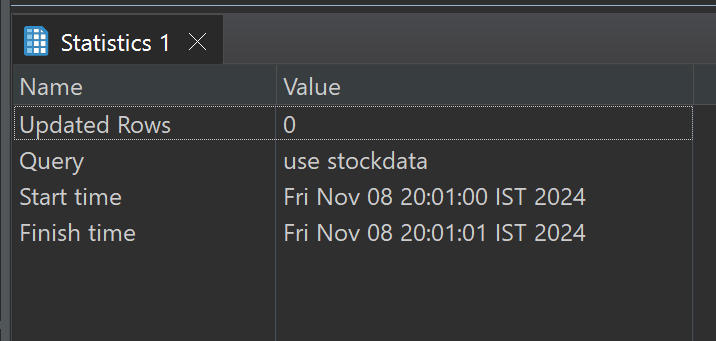
\includegraphics[width=0.45\textwidth]{Images/Task2.png}
	\caption{Output of Task 2}
\end{figure}

\section*{Task 3}

\begin{task*}[3]
Get a schema dump of the table nsedata using SQL
\end{task*}

\begin{lstlisting}[language=SQL, caption=Schema Dump of Table nsedata]
SHOW CREATE TABLE nsedata;
\end{lstlisting}

% lstlisting for normal text
\begin{lstlisting}[caption=Schema Dump of Table nsedata]
CREATE TABLE `nsedata` (
  `symbol` varchar(50) CHARACTER SET utf8mb4 COLLATE utf8mb4_0900_ai_ci NOT NULL,
  `series` varchar(50) CHARACTER SET utf8mb4 COLLATE utf8mb4_0900_ai_ci NOT NULL,
  `open` decimal(20,6) NOT NULL,
  `high` decimal(20,6) NOT NULL,
  `low` decimal(20,6) NOT NULL,
  `close` decimal(20,6) NOT NULL,
  `last` decimal(20,6) NOT NULL,
  `prevclose` decimal(20,6) NOT NULL,
  `tottrdqty` int NOT NULL,
  `tottrdval` decimal(20,6) NOT NULL,
  `timestamp` varchar(50) CHARACTER SET utf8mb4 COLLATE utf8mb4_0900_ai_ci NOT NULL,
  `anum` mediumint DEFAULT NULL,
  `isin` varchar(50) DEFAULT NULL,
  `extra` varchar(50) DEFAULT NULL
) 
ENGINE=InnoDB DEFAULT CHARSET=utf8mb4 COLLATE=utf8mb4_0900_ai_ci COMMENT='Table containing stock data obtained from NSE'
\end{lstlisting}

\clearpage

\section*{Task 4}

\begin{task*}[4]
Get a count of the total number of records in nsedata
\end{task*}

\begin{lstlisting}[language=SQL, caption=Counting the Total Number of Records]
SELECT COUNT(*) FROM nsedata;
\end{lstlisting}

\begin{figure}[H]
	\centering
	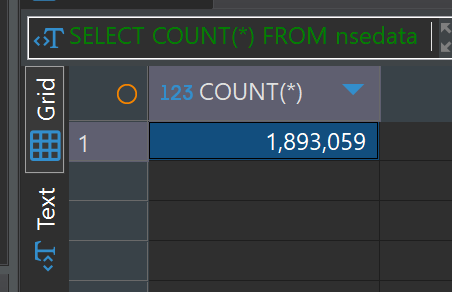
\includegraphics[width=0.45\textwidth]{Images/Task4.png}
	\caption{Output of Task 4}
\end{figure}

\section*{Task 5}

\begin{task*}[5]
Get the total count of the records for the month "October 2012"
\end{task*}

\begin{lstlisting}[language=SQL, caption=Counting the Total Number of Records for October 2012]
SELECT COUNT(*)
FROM nsedata
WHERE STR_TO_DATE(timestamp,'%d-%b-%Y')
BETWEEN '2012-10-01'
AND '2012-10-31';
\end{lstlisting}

\begin{figure}[H]
	\centering
	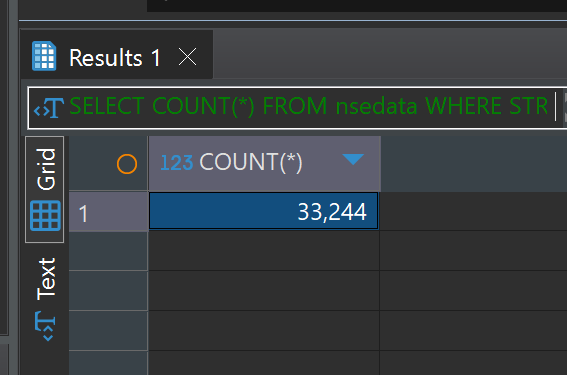
\includegraphics[width=0.45\textwidth]{Images/Task5.png}
	\caption{Output of Task 5}
\end{figure}

\section*{Task 6}

\begin{task*}[6]
Repeat `4', but only for the stock with symbol “GEOMETRIC”
\end{task*}

\begin{lstlisting}[language=SQL, caption=Counting the Total Number of Records for GEOMETRIC]
SELECT COUNT(*)
FROM nsedata
WHERE symbol = 'GEOMETRIC';
\end{lstlisting}

\begin{figure}[H]
	\centering
	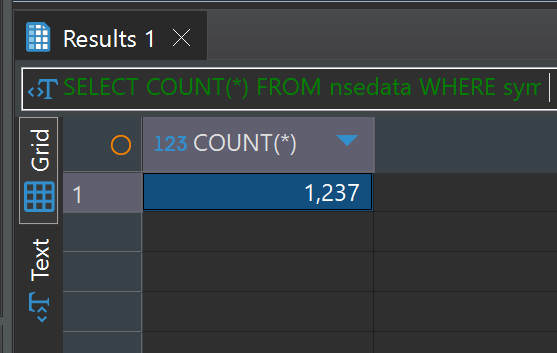
\includegraphics[width=0.45\textwidth]{Images/Task6.png}
	\caption{Output of Task 6}
\end{figure}

\section*{Task 7}

\begin{task*}[7]
Repeat `6', but only display the first 10 records
\end{task*}

\begin{lstlisting}[language=SQL, caption=Displaying the First 10 Records for GEOMETRIC]
SELECT *
FROM nsedata
WHERE symbol = 'GEOMETRIC' 
LIMIT 10;
\end{lstlisting}

\begin{figure}[H]
	\centering
	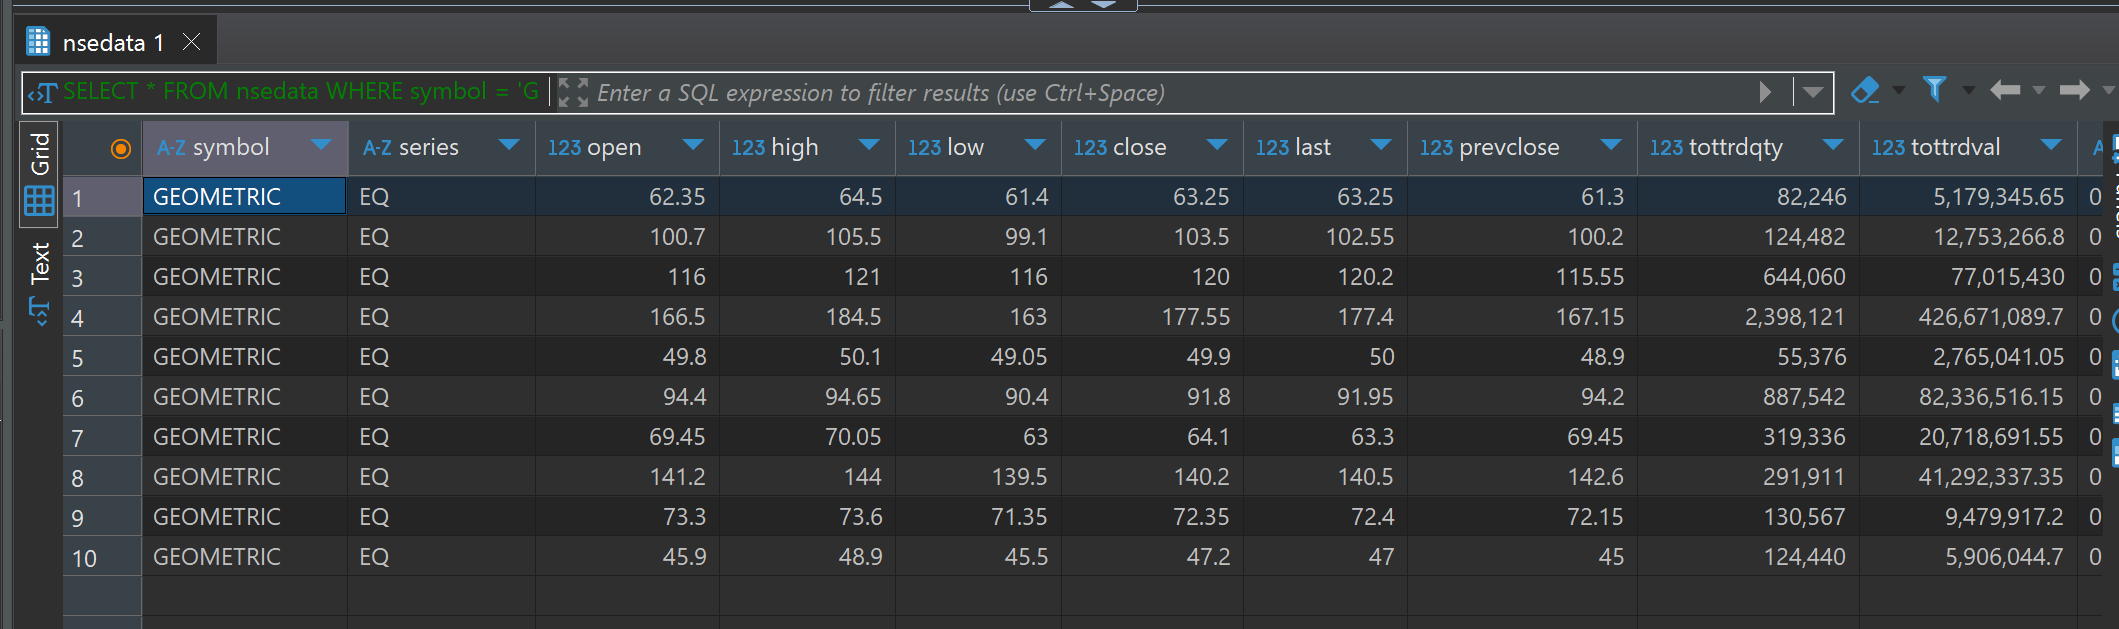
\includegraphics[width=0.45\textwidth]{Images/Task7.png}
	\caption{Output of Task 7}
\end{figure}

\clearpage

\section*{Task 8}

\begin{task*}[8]
Totally, how many records of "INFY" does the table contain?
\end{task*}

\begin{lstlisting}[language=SQL, caption=Counting the Total Number of Records for INFY]
SELECT COUNT(*)
FROM nsedata
WHERE symbol = 'INFY';
\end{lstlisting}

\begin{figure}[H]
	\centering
	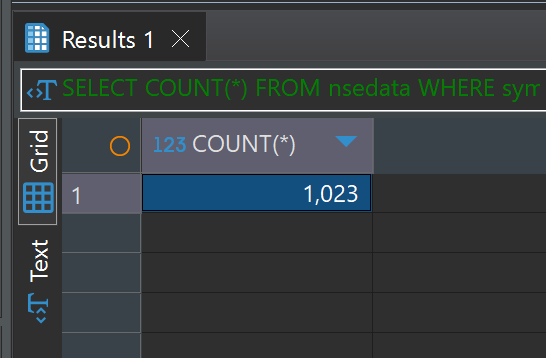
\includegraphics[width=0.45\textwidth]{Images/Task8.png}
	\caption{Output of Task 8}
\end{figure}

\section*{Task 9}

\begin{task*}[9]
Get a listing of the first $10$ records of "3IINFOTECH", but the listing should contain only the following columns: symbol, open, high, low, close, and timestamp
\end{task*}

\begin{lstlisting}[language=SQL, caption=Displaying the First 10 Records for 3IINFOTECH]
SELECT symbol, open, high, low, close,
Timestamp
FROM nsedata
WHERE symbol = '3IINFOTECH'
LIMIT 10;
\end{lstlisting}

\begin{figure}[H]
	\centering
	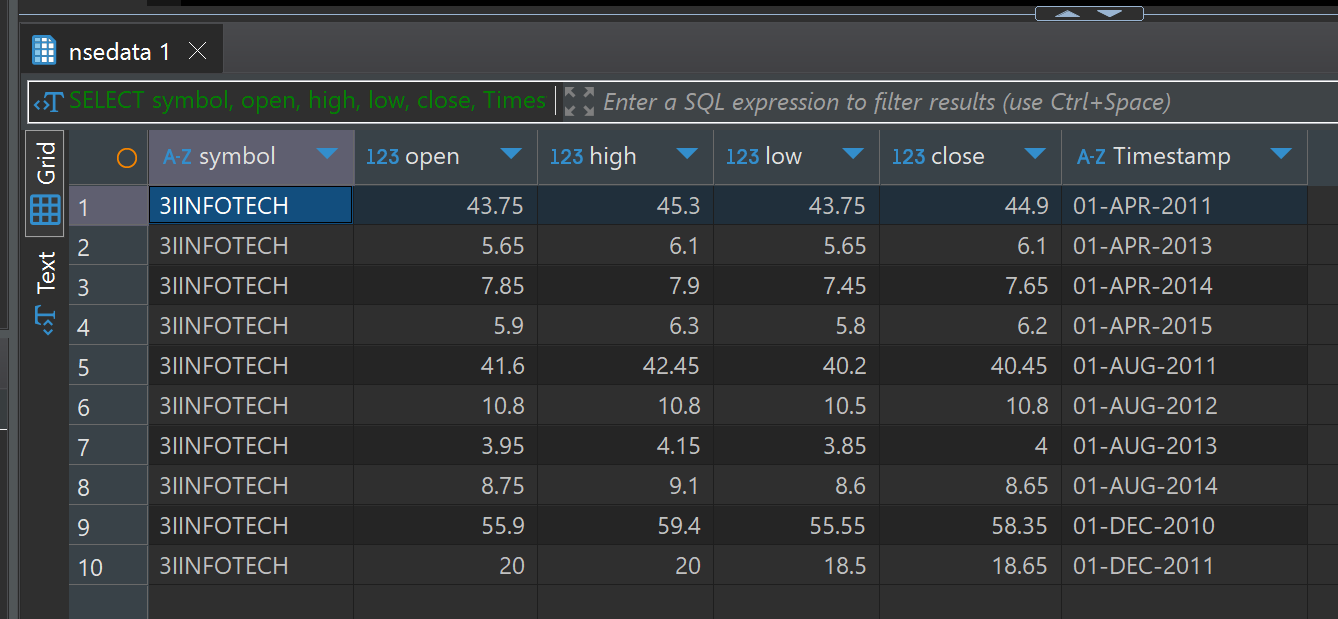
\includegraphics[width=0.45\textwidth]{Images/Task9.png}
	\caption{Output of Task 9}
\end{figure}

\clearpage

\section*{Task 10}

\begin{task*}[10]
Repeat `9', but this time use the results to create a table \textbf{t1} in the \textbf{stockdata} database
\end{task*}

\begin{lstlisting}[language=SQL, caption=Creating Table t1]
CREATE TABLE t1 AS
SELECT symbol, open, high, low, close, timestamp
FROM nsedata
WHERE symbol = '3IINFOTECH'
LIMIT 10;
SHOW TABLES;
\end{lstlisting}

\begin{figure}[H]
	\centering
	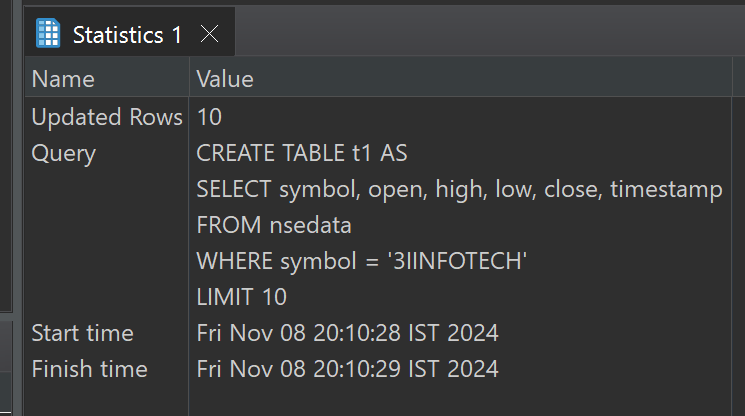
\includegraphics[width=0.45\textwidth]{Images/Task10-1.png}
	\caption{Output of Task 10}
\end{figure}

\begin{figure}[H]
	\centering
	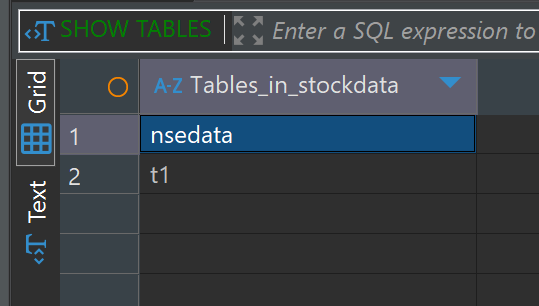
\includegraphics[width=0.45\textwidth]{Images/Task10-2.png}
	\caption{Output of Task 10}
\end{figure}

\clearpage

\section*{Task 11}

\begin{task*}[11]
Using \textbf{t1} find out the following for the column \textbf{close}: max, min, mean. standard deviation and variance
\end{task*}

\begin{lstlisting}[language=SQL, caption=Finding Statistics for the close Column]
SELECT MAX(close) AS max_close, MIN(close) AS min_close, AVG(close) AS mean_close, STDDEV(close) AS stddev_close, VARIANCE(close) AS variance_close
FROM t1;
\end{lstlisting}

\begin{figure}[H]
	\centering
	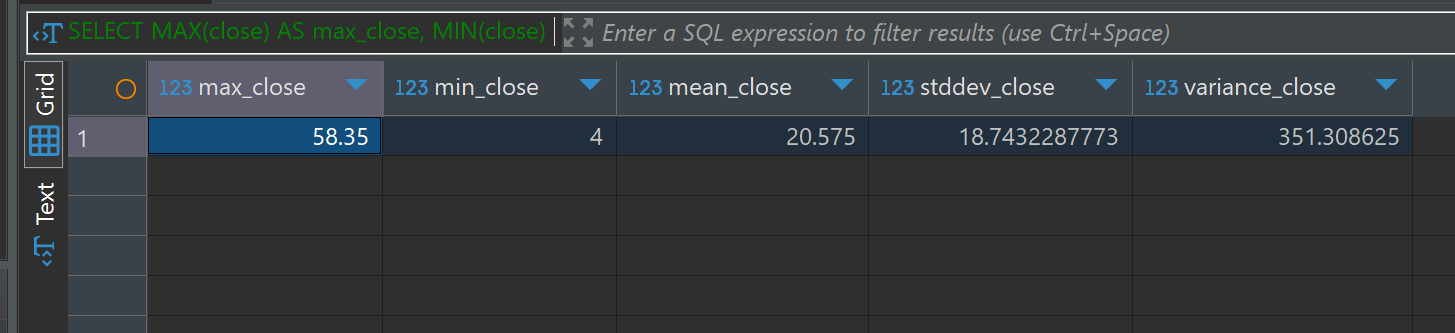
\includegraphics[width=0.45\textwidth]{Images/Task11.png}
	\caption{Output of Task 11}
\end{figure}

\section*{Task 12}

\begin{task*}[12]
How will you find out the value of the median, if that is also required?
\end{task*}

\begin{lstlisting}[language=SQL, caption=Finding the Median for the close Column]
SET @row_number := 0;

SELECT AVG(close) AS median_close
FROM (
  SELECT close,
     @row_number := @row_number + 1 AS row_num
  FROM t1
  ORDER BY close
) AS sorted_data

WHERE row_num IN (
  FLOOR((@row_number + 1) / 2),
  CEIL((@row_number + 1) / 2)
);
\end{lstlisting}

\begin{figure}[H]
	\centering
	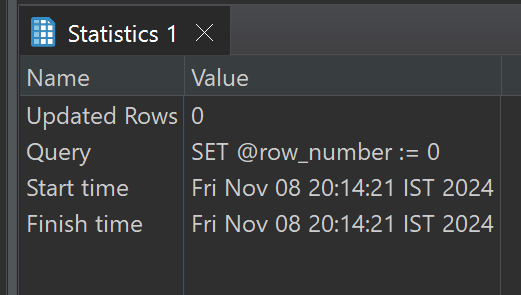
\includegraphics[width=0.45\textwidth]{Images/Task12-1.png}
	\caption{Output of Task 12}
\end{figure}

\begin{figure}[H]
	\centering
	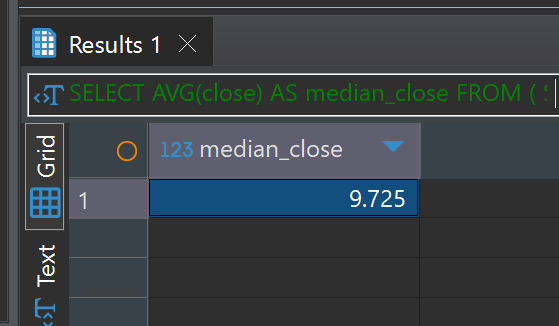
\includegraphics[width=0.45\textwidth]{Images/Task12-2.png}
	\caption{Output of Task 12}
\end{figure}

\section*{Task 13}

\begin{task*}[13]
Delete table \textbf{t1}
\end{task*}

\begin{lstlisting}[language=SQL, caption=Deleting Table t1]
DROP TABLE t1;
SHOW TABLES;
\end{lstlisting}

\begin{figure}[H]
	\centering
	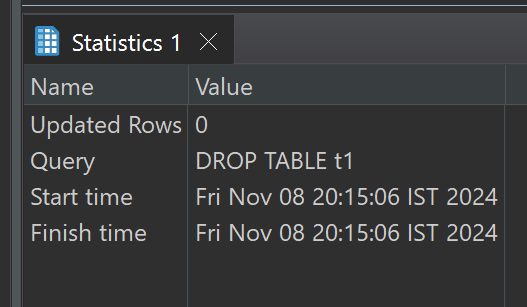
\includegraphics[width=0.4\textwidth]{Images/Task13-1.png}
	\caption{Output of Task 13}
\end{figure}

\begin{figure}[H]
	\centering
	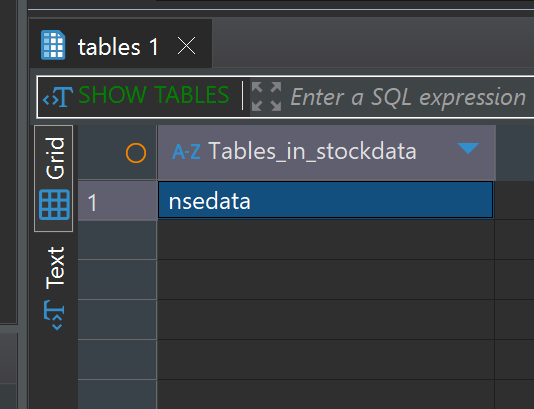
\includegraphics[width=0.4\textwidth]{Images/Task13-2.png}
	\caption{Output of Task 13}
\end{figure}

% \clearpage

\section*{Task 14}

\begin{task*}[14]
Switch back to using nsedata. Using the GROUP BY functionality of SQL create a table \textbf{t2} containing the average value of \textbf{close} for every symbol in the table. Hint: the table will have the columns: \textbf{symbol}, \textbf{average}
\end{task*}

\begin{lstlisting}[language=SQL, caption=Creating Table t2]
CREATE TABLE t2 AS
SELECT symbol, AVG(close) AS average_close
FROM nsedata
GROUP BY symbol;
SELECT * FROM t2;
\end{lstlisting}

\begin{figure}[H]
	\centering
	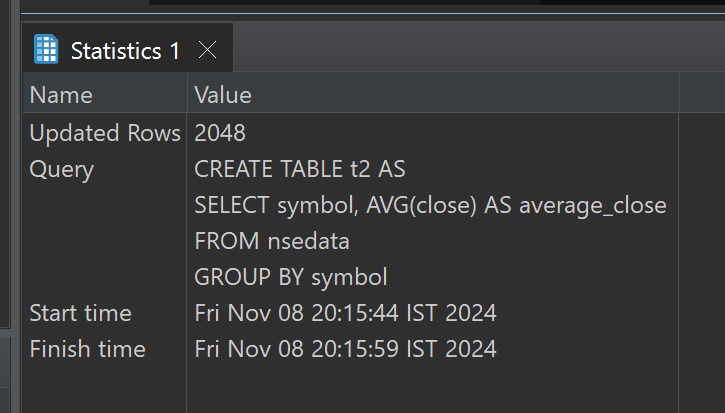
\includegraphics[width=0.45\textwidth]{Images/Task14-1.png}
	\caption{Output of Task 14}
\end{figure}

\begin{figure}[H]
	\centering
	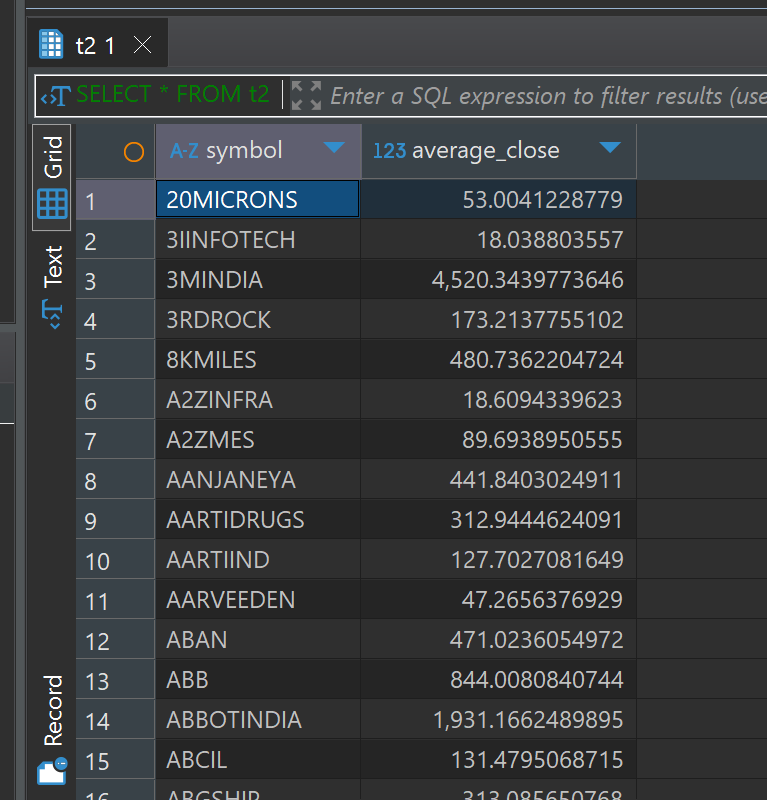
\includegraphics[width=0.45\textwidth]{Images/Task14-2.png}
	\caption{Output of Task 14}
\end{figure}

\clearpage

\section*{Task 15}

\begin{task*}[15]
Create a table \textbf{t3} such that it contains the following columns: symbol, open, close, "average of open and close". Fill up this table for the company GEOMETRIC, for the month of October 2012
\end{task*}

\begin{lstlisting}[language=SQL, caption=Creating Table t3]
CREATE TABLE t3 AS
SELECT symbol, open, close, (open + close) / 2 AS avg_open_close
FROM nsedata
WHERE symbol = 'GEOMETRIC'
AND STR_TO_DATE(timestamp, '%d-%b-%Y')
BETWEEN '2012-10-01' AND '2012-10-31';
SELECT * FROM t3;
\end{lstlisting}

\begin{figure}[H]
	\centering
	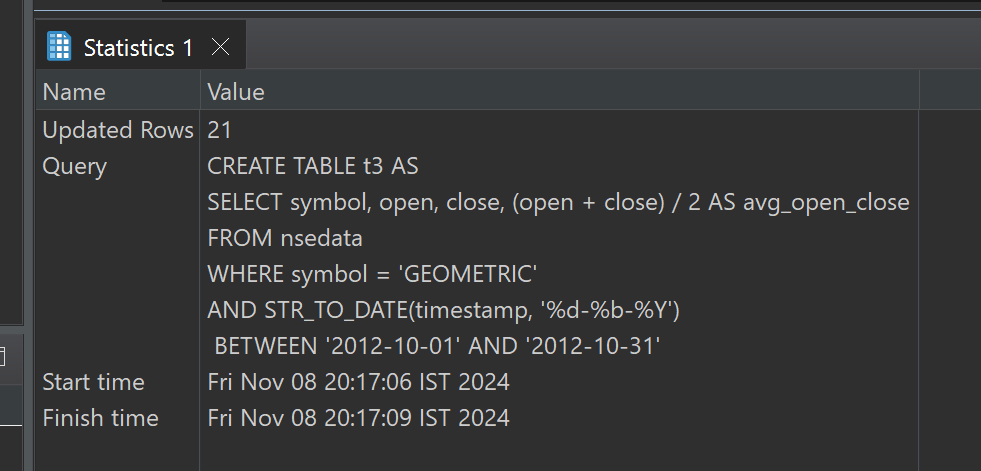
\includegraphics[width=0.5\textwidth]{Images/Task15-1.png}
	\caption{Output of Task 15}
\end{figure}

\begin{figure}[H]
	\centering
	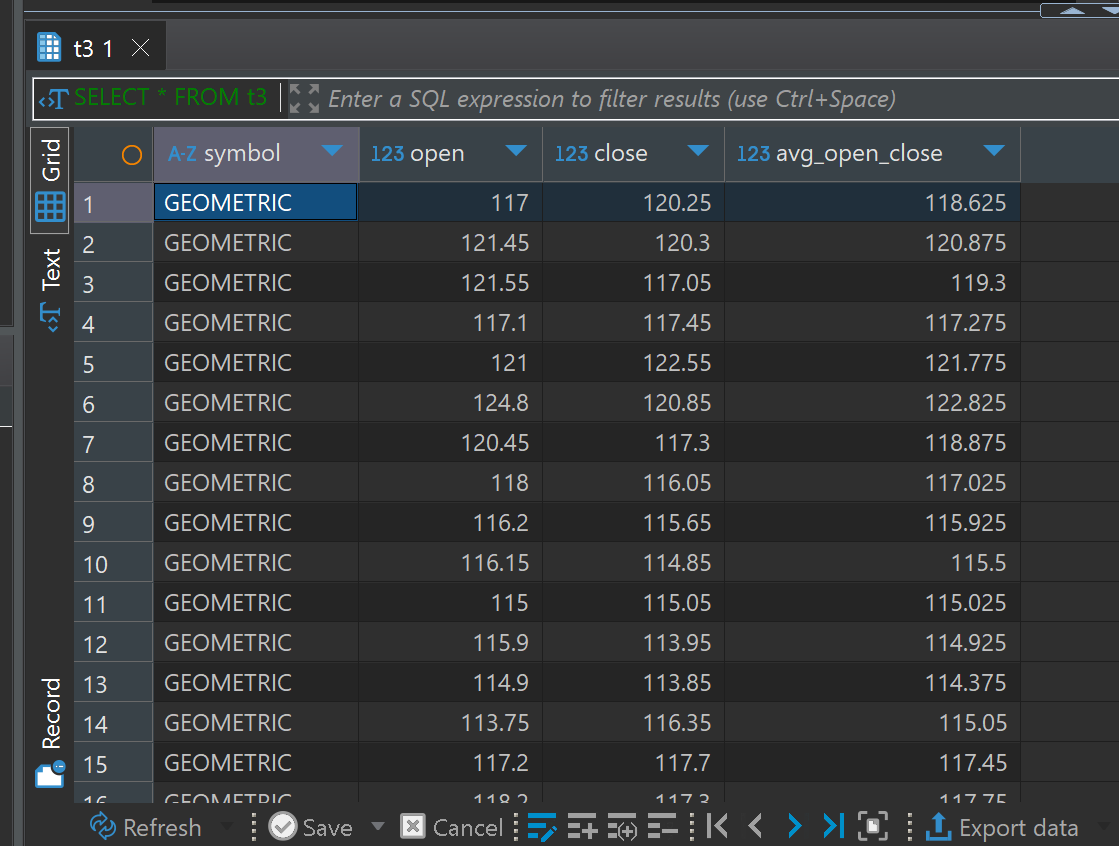
\includegraphics[width=0.5\textwidth]{Images/Task15-2.png}
	\caption{Output of Task 15}
\end{figure}

\clearpage

\section*{Task 16}

\begin{task*}[16]
It is required to create a table \textbf{t4} such that it contains the data for two companies \textbf{GEOMETRIC} and \textbf{TCS}. The columns of this table should be as follows: timestamp, close\_tcs, close\_geometric. \\
Hint: use JOIN
\end{task*}

\begin{lstlisting}[language=SQL, caption=Creating Table t4]
CREATE TABLE t4 AS
SELECT tab1.timestamp, tab1.close AS close_tcs, tab2.close AS close_geometric
FROM nsedata tab1
JOIN nsedata tab2
ON tab1.timestamp = tab2.timestamp
WHERE tab1.symbol = 'TCS'
AND tab2.symbol = 'GEOMETRIC';
SELECT * FROM t4;
\end{lstlisting}

\begin{figure}[H]
	\centering
	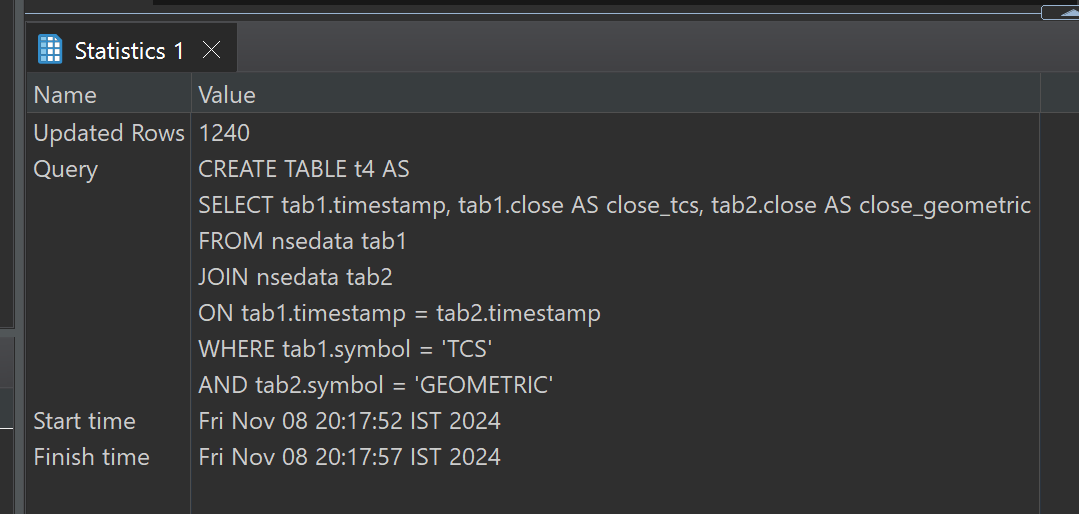
\includegraphics[width=0.45\textwidth]{Images/Task16-1.png}
	\caption{Output of Task 16}
\end{figure}

\begin{figure}[H]
	\centering
	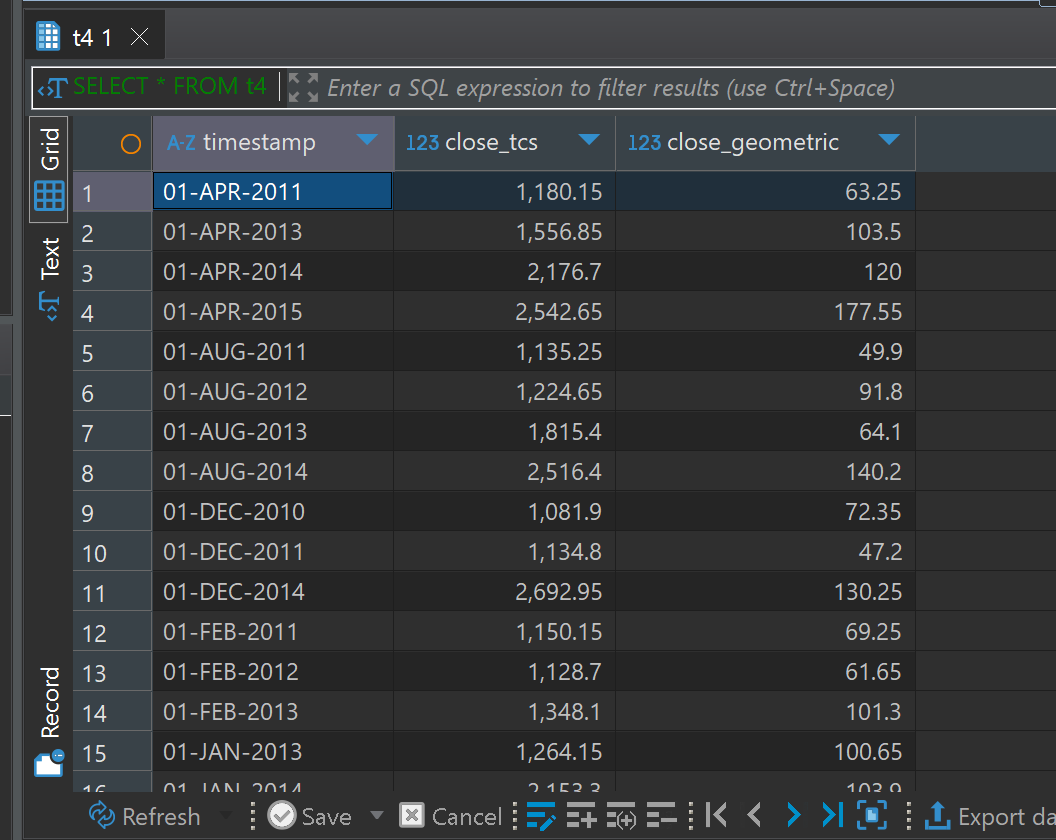
\includegraphics[width=0.45\textwidth]{Images/Task16-2.png}
	\caption{Output of Task 16}
\end{figure}

\clearpage

\section*{Task 17}

\begin{task*}[17]
Find out the maximum and minimum difference in the daily closing prices of these two companies.
\end{task*}

\begin{lstlisting}[language=SQL, caption=Finding the Maximum and Minimum Difference in Closing Prices]
SELECT MAX(ABS(close_tcs - close_geometric)) AS max_diff, MIN(ABS(close_tcs - close_geometric)) AS min_diff
FROM t4;
\end{lstlisting}

\begin{figure}[H]
	\centering
	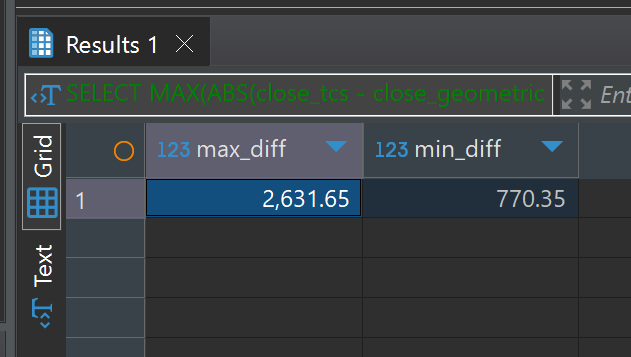
\includegraphics[width=0.4\textwidth]{Images/Task17.png}
	\caption{Output of Task 17}
\end{figure}

\section*{Task 18}

\begin{task*}[18]
Based on \textbf{t4} can you identify those days on which the difference in their closing price was more than the average of the minimum and maximum differences of their closing prices.
\end{task*}

\begin{lstlisting}[language=SQL, caption=Identifying Days with Closing Price Difference More than Average]
SELECT timestamp, close_tcs, close_geometric, ABS(close_tcs - close_geometric) AS daily_diff
FROM t4
WHERE ABS(close_tcs - close_geometric) > (SELECT (MAX(ABS(close_tcs - close_geometric)) + MIN(ABS(close_tcs - close_geometric))) / 2
FROM t4
);
\end{lstlisting}

\begin{figure}[H]
	\centering
	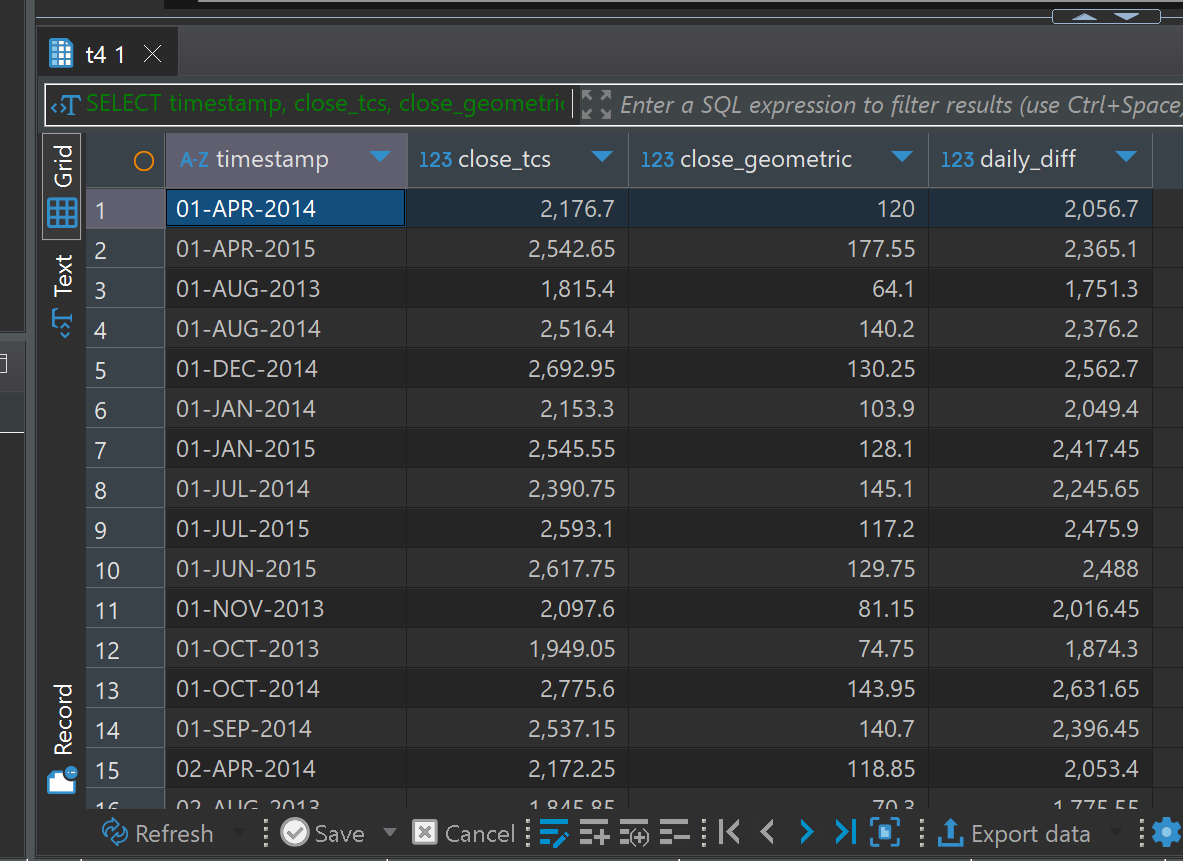
\includegraphics[width=0.4\textwidth]{Images/Task18.png}
	\caption{Output of Task 18}
\end{figure}

\section*{Task 19}

\begin{task*}[19]
Based on \textbf{nsedata}, create table \textbf{t5} such that it contains the average \textbf{close} price of each company traded in the month of April 2012. The table should be sorted in descending order of the average close price.
\end{task*}

\begin{lstlisting}[language=SQL, caption=Creating Table t5]
CREATE TABLE t5 AS
SELECT symbol, AVG(close) AS average_close
FROM nsedata
WHERE STR_TO_DATE(timestamp, '%d-%b-%Y')
BETWEEN '2012-04-01' AND '2012-04-30'
GROUP BY symbol
ORDER BY average_close DESC;
SELECT * FROM t5;
\end{lstlisting}

\begin{figure}[H]
	\centering
	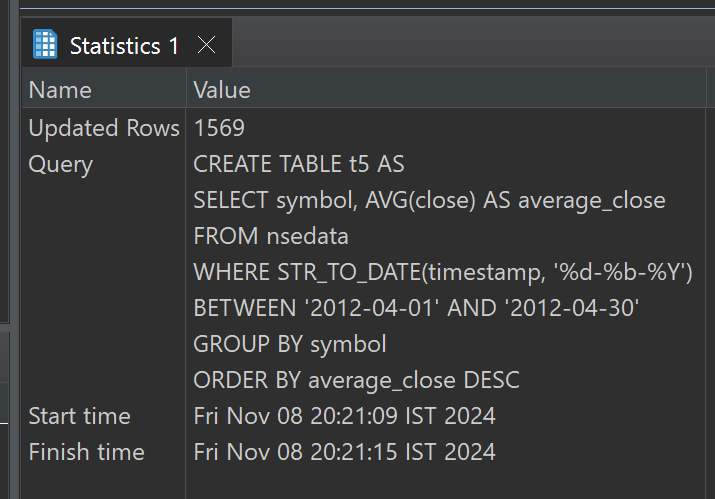
\includegraphics[width=0.4\textwidth]{Images/Task19-1.png}
	\caption{Output of Task 19}
\end{figure}

\begin{figure}[H]
	\centering
	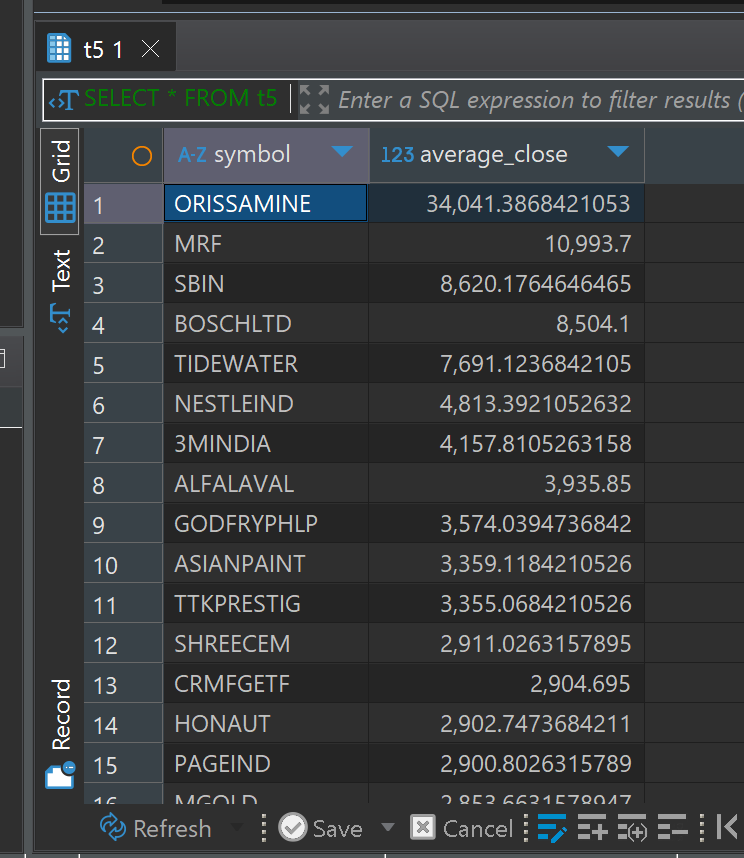
\includegraphics[width=0.4\textwidth]{Images/Task19-2.png}
	\caption{Output of Task 19}
\end{figure}

\section*{Task 20}

\begin{task*}[20]
Not all companies are traded every day. It is required to create a table that contains a count of the days each company has been traded in a selected year - say 2012. The table should be sorted in descending order of the count.
\end{task*}

\begin{lstlisting}[language=SQL, caption=Creating Table trade\_count]
CREATE TABLE trade_count AS
SELECT symbol, COUNT(DISTINCT DATE(STR_TO_DATE(timestamp, '%d-%b-%Y'))) AS trade_days
FROM nsedata
WHERE YEAR(STR_TO_DATE(timestamp,'%d-%b-%Y')) = 2012
GROUP BY symbol
ORDER BY trade_days DESC;
SELECT * FROM trade_count;
\end{lstlisting}

\begin{figure}[H]
	\centering
	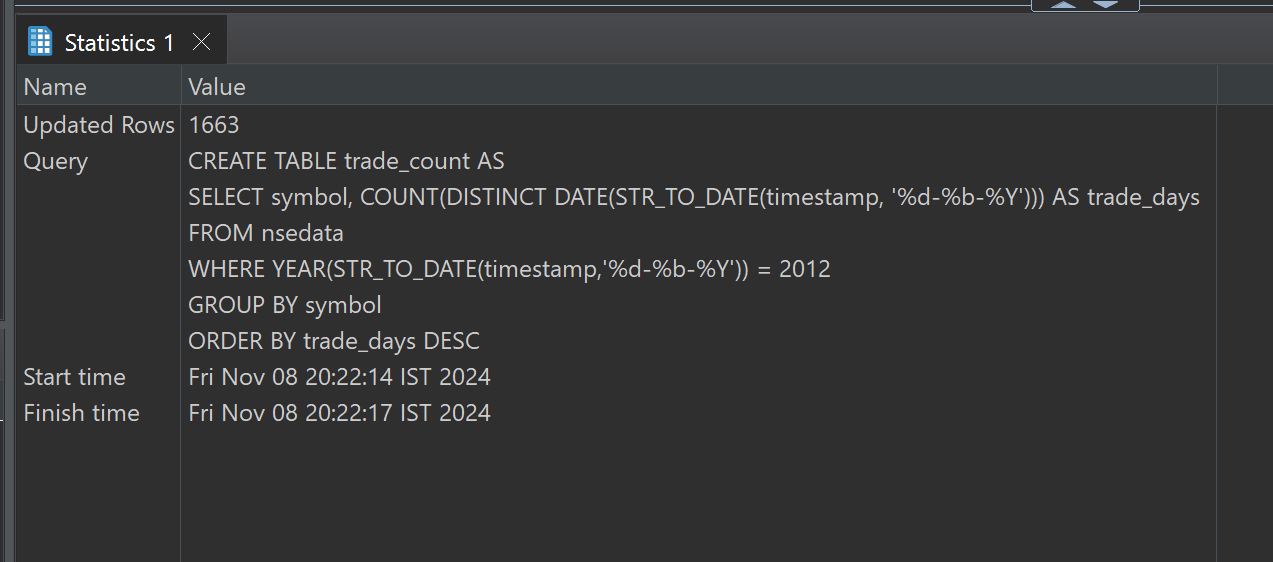
\includegraphics[width=0.45\textwidth]{Images/Task20-1.png}
	\caption{Output of Task 20}
\end{figure}

\begin{figure}[H]
	\centering
	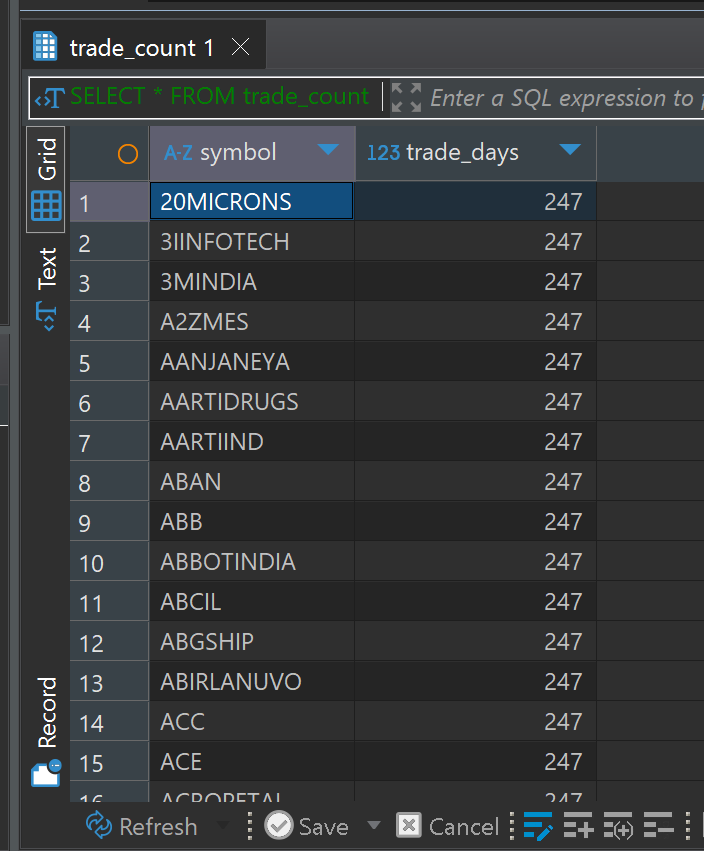
\includegraphics[width=0.45\textwidth]{Images/Task20-2.png}
	\caption{Output of Task 20}
\end{figure}

\end{document}